\chapter{MixVRTの実装}\label{cha:Implementation}
本章では、試作した\toolName の実装について説明する。
% なお、本研究で用いる、\toolName の各処理部が取得または生成する画像名を、以下に定義する。
% \begin{itemize}
%     \item 変更前画像
%     \item 変更後画像
%     \item 高解像度にした変更前画像
%     \item 高解像度にした変更後画像
%     \item 画像比較に基づく削除箇所を赤枠で囲むことで強調表示した、変更前画像
%     \item 画像比較に基づく追加箇所を緑枠で囲むことで強調表示した、変更後画像
%     \item HTMLコードにおけるbody要素内の追加とstyle要素内の追加のどちらか、
%           または両方の追加による変更を受けた箇所を赤枠で囲むことで強調表示した、変更前画像
%     \item HTMLコードにおけるbody要素内の削除とstyle要素内の削除のどちらか、
%           または両方の削除による変更を受けた箇所を緑枠で囲むことで強調表示した、変更後画像
%     \item HTMLコードの変更に基づく変更箇所を色付きの枠で囲むことで強調表示した、変更前画像
%     \item HTMLコードの変更に基づく変更箇所を色付きの枠で囲むことで強調表示した、変更後画像
%     \item レイアウトの不具合箇所を色付きの枠で囲むことで強調表示した、変更前画像
%     \item レイアウトの不具合箇所を色付きの枠で囲むことで強調表示した、変更後画像
% \end{itemize}
\par
\toolName のシステム構成を、図\ref{fig:System}に示す。
\begin{figure}[tp]
    \begin{center}
        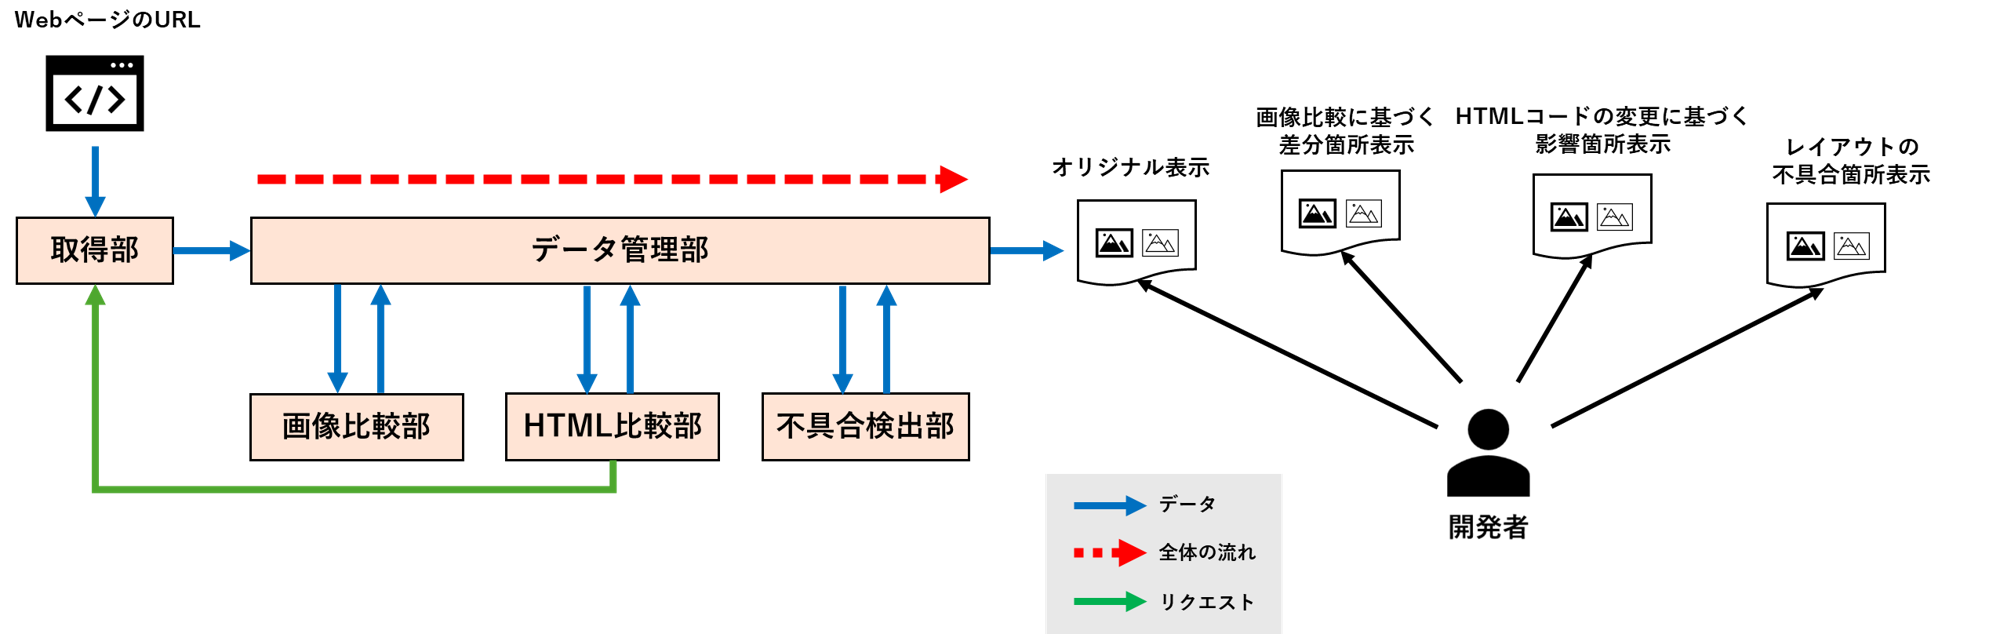
\includegraphics[width=1.0\columnwidth]{image/new_System.png}
        \caption{\toolName のシステム構成}
        \label{fig:System}
    \end{center}
\end{figure}
% 私の開発したツールは、まずユーザーがWebページのURLを入力します。
% このURLを受け取ると、ツールは該当するWebページから画像を取得し、
% これらの画像に対して特定の処理を行います。処理された画像は"static/images"ディレクトリに保持されます。
% そして、Flaskがローカルサーバを提供し、
% "templates"フォルダにあるHTMLコードが"static/images"ディレクトリを参照できるようになっています。
% この仕組みにより、ユーザーはローカルに立てられたFlaskサーバを通じて、
% Webページ上で生成された画像を確認することができます。
\toolName は、以下の5つの処理部から構成する。
\begin{itemize}
    \item データ管理部
    \item 取得部
    \item 画像比較部
    \item HTML比較部
    \item 不具合検出部
          % \item 表示部
          % \item 表示部
\end{itemize}
% \begin{itemize}
%     \item 取得部
%     \item 画像比較部
%           \begin{enumerate}
%               \item 差分箇所検出
%           \end{enumerate}
%     \item HTML比較部
%           \begin{enumerate}
%               \item 差分コード生成
%               \item 差分コード解析
%               \item 変更箇所強調HTMLコード生成
%           \end{enumerate}
%     \item レイアウト副作用箇所抽出部
%     \item 表示部
% \end{itemize}
以降、\toolName を構成する5つの処理部について説明する。
\par

\section{データ管理部}\label{sec:data_admin_section}
データ管理部は、システム内の各処理部間におけるデータの伝達を担い、他の処理部とのデータのやり取りとデータの保持を行う。
なお、本論文におけるデータとは、処理前後のWebページの画像やHTMLコードであり、
やり取りしたデータはデータ管理部が持つディレクトリに保持する。
また、取得部(\ref{sec:Web_data_get_section}節で後述)のみ、データ管理部とのデータのやり取りが一方向である(図\ref{fig:System}を参照)。
% また、取得部(\ref{sec:Web_data_get_section}節で後述)と表示部(\ref{sec:Interface_Display_Section}節で後述)のみ、データ管理部とのデータのやり取りが一方向である(図\ref{fig:System}を参照)。
% また、取得部とデータ管理部の間におけるデータのやり取りは、取得部からデータ管理部への一方向のみであり、
% データ管理部と表示部の間におけるデータのやり取りは、データ管理部から表示部への一方向のみである。
\par
データ管理部における最初のデータのやり取りの相手は、取得部である。
取得部からデータを受け取ると、そのデータをデータ管理部のbase\_dirディレクトリ(後述)に保持する。
保持した後、\toolName の初期設定時の場合、
% Flaskを用いて構築したローカルサーバ上で動作するWebページ(
\toolName が生成した画像を閲覧できるWebページ(\ref{sec:Flask}節を参照)に、
変更前画像のみを出力し、全体の処理を終了する。
\toolName の初期設定時ではない場合、取得部に続き、
画像比較部(\ref{sec:Difference_extraction_section}節で後述)、HTML比較部(\ref{sec:Affected_area_extraction}節で後述)、不具合検出部(\ref{sec:Layout_bug_extraction_section}節で後述)の順に
データのやり取りを行う。やり取りしたデータはデータ管理部のdiff\_dirディレクトリ(後述)に保持する。
\par
各処理部とのやり取りを終えると、
データ管理部は、\toolName が生成した画像を閲覧できるWebページに、
\ref{subsec:MixVRT_IO}節で述べた8つのPNG形式の画像を出力し、全体の処理を終了する。
% なお、出力先のWebページは、\toolName による視覚的回帰テストで生成した画像の確認が効率的に行えるWebページを開発者に提供する。
\par
各処理部との間でやり取りしたデータを保持する各ディレクトリを、以下に示す。
\begin{itemize}
    \item base\_dirディレクトリ:\\
          取得部でやり取りしたデータを保持する。
          base\_dirディレクトリに保持するデータの詳細を、表\ref{tb: base_dir_data}に示す。
          表\ref{tb: base_dir_data}中の変更後画像と変更後HTMLコードに関しては、
          \toolName の3回目以降の実行時は、前回実行時の変更後画像と変更後HTMLコードが存在するため、
          そのデータを削除してから、新たに、変更後画像と変更後HTMLコードを保持する。
          また、表\ref{tb: base_dir_data}中の変更前画像と変更前HTMLコードに関しては、
          開発者が「\$ make save」(\ref{subsec:MixVRT_evaluate}を参照)を実行することで、
          変更後画像と変更後HTMLコードを、それぞれ変更前画像と変更前HTMLコードとして更新する。
    \item diff\_dirディレクトリ:\\
          画像比較部、HTML比較部、不具合検出部とやり取りしたデータを保持する。
          diff\_dirディレクトリに保持するデータの詳細を、表\ref{tb: diff_dir_data}に示す。
\end{itemize}
% \item disp\_dirディレクトリ:\\
%       表示部に出力するデータを保持する。
% 変更前画像と変更後画像、Webページの変更前HTMLコードと変更後HTMLコードを用いて、
\begin{table}[tp]
    \caption{base\_dirディレクトリに保持するデータの詳細}
    \label{tb: base_dir_data}
    \centering
    \begin{tabular}{c|l}
        \hline
        データ           & \multicolumn{1}{c}{説明}                                   \\
        \hline \hline
        変更前画像       & \toolName の初期設定時に取得するWebページの画像            \\ \hline
        変更前HTMLコード & \toolName の初期設定時に取得するWebページのHTMLコード      \\ \hline
        変更後画像       & \toolName の2回目以降実行時に取得するWebページの画像       \\ \hline
        変更後HTMLコード & \toolName の2回目以降実行時に取得するWebページのHTMLコード \\ \hline
    \end{tabular}
\end{table}

\begin{table}[tp]
    \caption{diff\_dirディレクトリに保持するデータの詳細}
    \label{tb: diff_dir_data}
    \centering
    % \fontsize{13pt}{3pt}\selectfont
    % \tiny
    % \scriptsize
    \footnotesize
    % \small
    % \normalsize
    % \large
    % \Large
    % \LARGE
    % \huge
    % \Huge
    \begin{tabular}{p{0.25\linewidth}|p{0.65\linewidth}}
        \hline
        \multicolumn{1}{c|}{データ} & \multicolumn{1}{c}{説明}                                                                                                              \\
        \hline \hline
        変更前高解像度画像          & 変更前画像を高解像度にした画像                                                                                                        \\ \hline
        変更後高解像度画像          & 変更後画像を高解像度にした画像                                                                                                        \\ \hline
        変更前高解像度二値化画像    & 変更前高解像度画像を二値化した画像                                                                                                    \\ \hline
        変更後高解像度二値化画像    & 変更後高解像度画像を二値化した画像                                                                                                    \\ \hline
        削除箇所二値化画像          & 変更前高解像度二値化画像から変更後高解像度二値化画像を引いた画像                                                                      \\ \hline
        追加箇所二値化画像          & 変更後高解像度二値化画像から変更前高解像度二値化画像                                                                     を引いた画像 \\ \hline
        削除箇所強調二値化画像      & 削除箇所二値化画像の白い部分を強調した画像                                                                                            \\ \hline
        追加箇所強調二値化画像      & 追加箇所二値化画像の白い部分を強調した画像                                                                                            \\ \hline
        差分箇所赤枠強調マスク画像  & 削除箇所強調二値化画像の白い部分を囲む赤枠のみを抽出した画像                                                                          \\ \hline
        差分箇所緑枠強調マスク画像  & 追加箇所強調二値化画像の白い部分を囲む緑枠のみを抽出した画像                                                                          \\ \hline    
        差分箇所変更前画像          & 変更により削除された範囲を、赤枠で囲むことで強調表示した、           Webページの変更前画像                                            \\ \hline
        差分箇所変更後画像          & 変更により追加された範囲を、緑枠で囲むことで強調表示した、           Webページの変更後画像                                            \\ \hline
        枠付き変更前HTMLコード      & 変更箇所における削除または変更があった画面要素を                     赤枠で囲むCSSクラスを付加した変更前HTMLコード                    \\ \hline
        枠付き変更後HTMLコード      & 変更箇所における追加または変更があった画面要素を                     緑枠で囲むCSSクラスを付加した変更後HTMLコード                    \\ \hline
        枠付き変更前画像            & 
        
        枠付き変更前HTMLコードをWebページとして表示した画面をスクリーンショットした画像                                                                       
        \\  \hline                                         
        枠付き変更後画像            & 
        
        枠付き変更後HTMLコードをWebページとして表示した画面をスクリーンショットした画像                                                                       
        \\  \hline                                               
        変更箇所赤枠強調マスク画像  & 枠付き変更前画像から赤枠のみを抽出した画像                                                                                            \\ \hline
        変更箇所緑枠強調マスク画像  & 枠付き変更後画像から緑枠のみを抽出した画像                                                                                            \\ \hline
        変更箇所変更前画像          & 変更により削除された画面要素の範囲を、赤枠で囲むことで強調表示した、 Webページの変更前画像                                            \\ \hline
        変更箇所変更後画像          & 変更により追加された画面要素の範囲を、緑枠で囲むことで強調表示した、 Webページの変更後画像                                            \\ \hline
        不具合箇所変更前画像        & レイアウトの不具合箇所のうち、削除したのに削除されていない箇所を、   赤枠で囲むことで強調表示した、Webページの変更前画像              \\ \hline
        不具合箇所変更後画像        & レイアウトの不具合箇所のうち、追加したのに追加されていない箇所を、   緑枠で囲むことで強調表示した、Webページの変更後画像              \\ \hline
    \end{tabular}
\end{table}

\section{取得部}\label{sec:Web_data_get_section}
取得部は、コマンドライン上から入力対象とするWebページのURLを入力として受け取り、URLから取得したWebページの画像とHTMLコードをデータ管理部のbase\_dirディレクトリに出力する。
なお、HTML比較部から取得部に、枠付きWebページのURL(\ref{sec:Flask}節を参照)を渡して呼び出す場合があり(図\ref{fig:System}と\ref{sec:Affected_area_extraction}節を参照)、
その場合は、取得した画像をデータ管理部のdiff\_dirディレクトリに出力する。
\par
Webページの画像取得は、Selenium WebDriver(\ref{sec:Selenium_WebDriver}節を参照)を用いて、WebページのURLからWebページの画像を取得する。
なお、取得するWebページの画像は、フルページのスクリーンショット画像である。
WebページのHTMLコード取得は、Pythonライブラリであるrequests(\ref{sec:requests}節を参照)を用いて、
WebページのURLからWebページのHTMLコードを取得する。

\section{画像比較部}\label{sec:Difference_extraction_section}
画像比較部は、データ管理部のbase\_dirディレクトリから変更前画像と変更後画像を受け取り、
「差分箇所変更前後画像」を生成する。
また、それらの画像から枠のみを残してそれ以外の部分を黒くすることで、差分箇所を囲む色付きの枠のみを抽出した、
「差分箇所赤枠強調マスク画像」と「差分箇所緑枠強調マスク画像」を生成する。
生成したマスク画像は、不具合検出部(\ref{sec:Layout_bug_extraction_section}節で後述)でレイアウトの不具合箇所を検出する際に用いる。
\par
画像比較部の処理の流れを、以下に示す。
\begin{enumerate}
    \item 高解像度画像生成処理
    \item 適応的二値化処理
    \item 差分検出処理
    \item 膨張処理
    \item 輪郭検出処理
    \item 枠描画処理
\end{enumerate}
また、\toolName の入力対象とする変更前画像と変更後画像の例を、図\ref{fig: img_original_bf_af}に示す。
\begin{figure}[tp]
    \begin{center}
        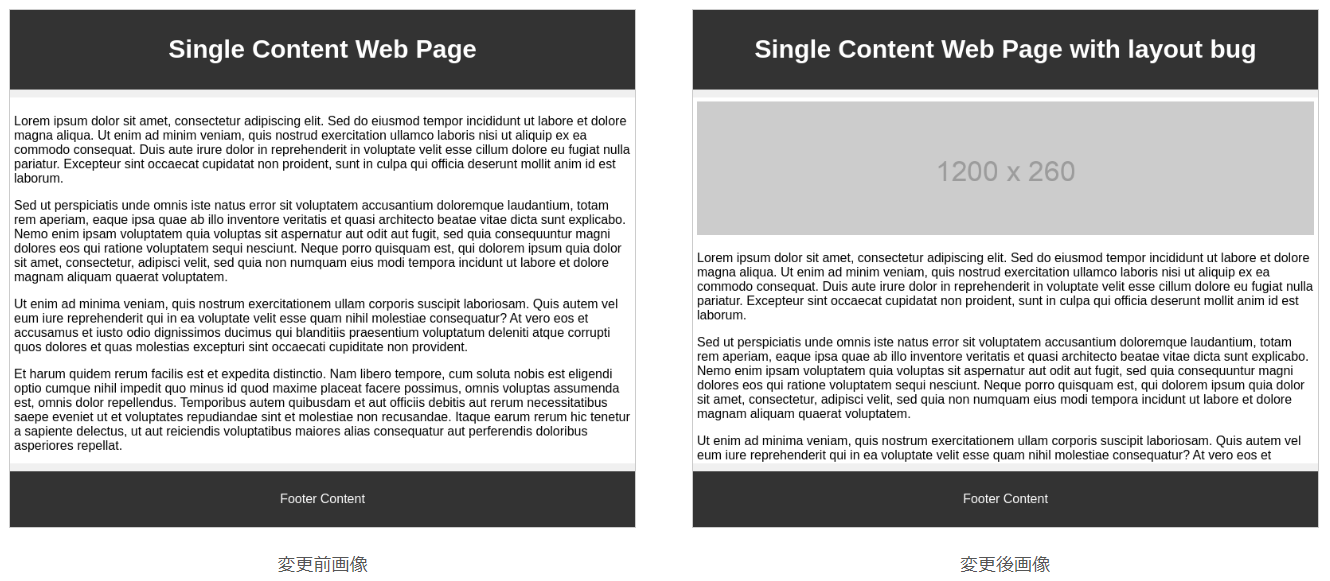
\includegraphics[width=1.0\columnwidth]{image/4_img_original_bf_af.png}
        \caption{\toolName の入力対象とする変更前画像(左)と変更後画像(右)の例}
        \label{fig: img_original_bf_af}
    \end{center}
\end{figure}
以降、画像比較部の各処理について説明する。
% 以降、図\ref{fig: img_original_bf_af}を例として、画像比較部の各処理について説明する。

\subsection{高解像度画像生成処理}\label{subsec:Generate_high_images}
高解像度画像生成処理は、変更前画像と変更後画像をそれぞれ高解像度画像にした、「変更前高解像度画像」と「変更後高解像度画像」を生成する。
高解像度にする前のテキスト画像と高解像度にした後のテキスト画像の例を、図\ref{fig: high_compare}に示す。
\begin{figure}[tp]
    \begin{center}
        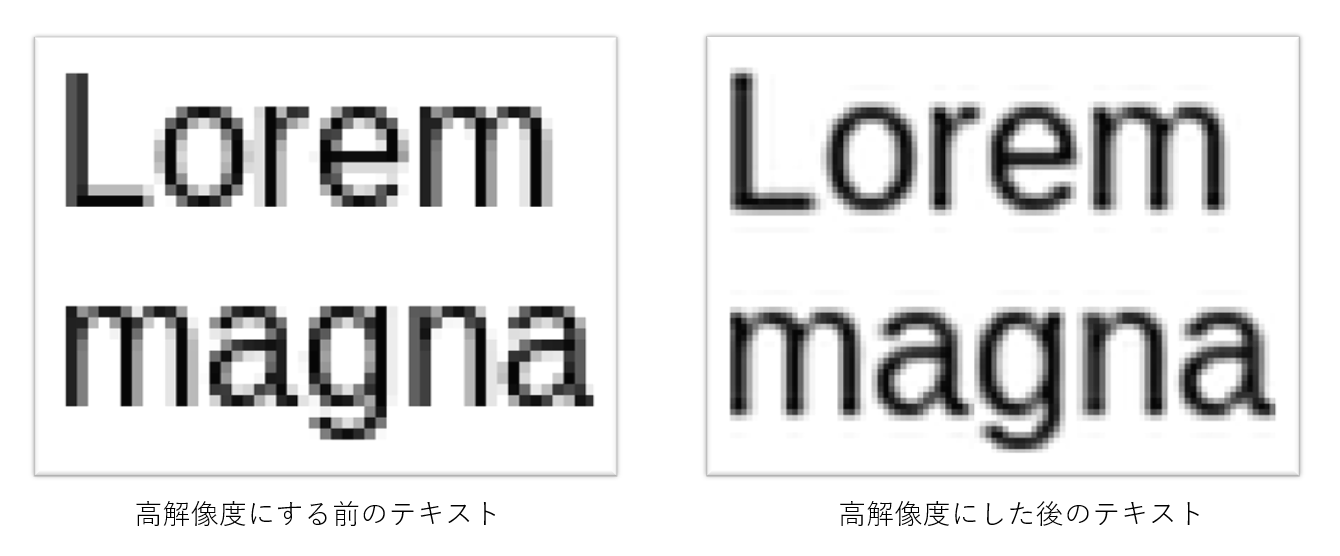
\includegraphics[width=1.0\columnwidth]{image/4_high_compare.png}
        \caption{高解像度にする前のテキスト画像(左)と高解像度にした後のテキスト画像(右)}
        \label{fig: high_compare}
    \end{center}
\end{figure}
この処理は、輪郭検出処理(\ref{subsec:contour_detection_processing}節で後述)の精度を向上するために必要である。
図\ref{fig: img_original_bf_af}に示した、変更前画像と変更後画像に高解像度画像生成処理を適用して生成した
「変更前高解像度画像」と「変更後高解像度画像」を、図\ref{fig: high_img}に示す。
\begin{figure}[tp]
    \begin{center}
        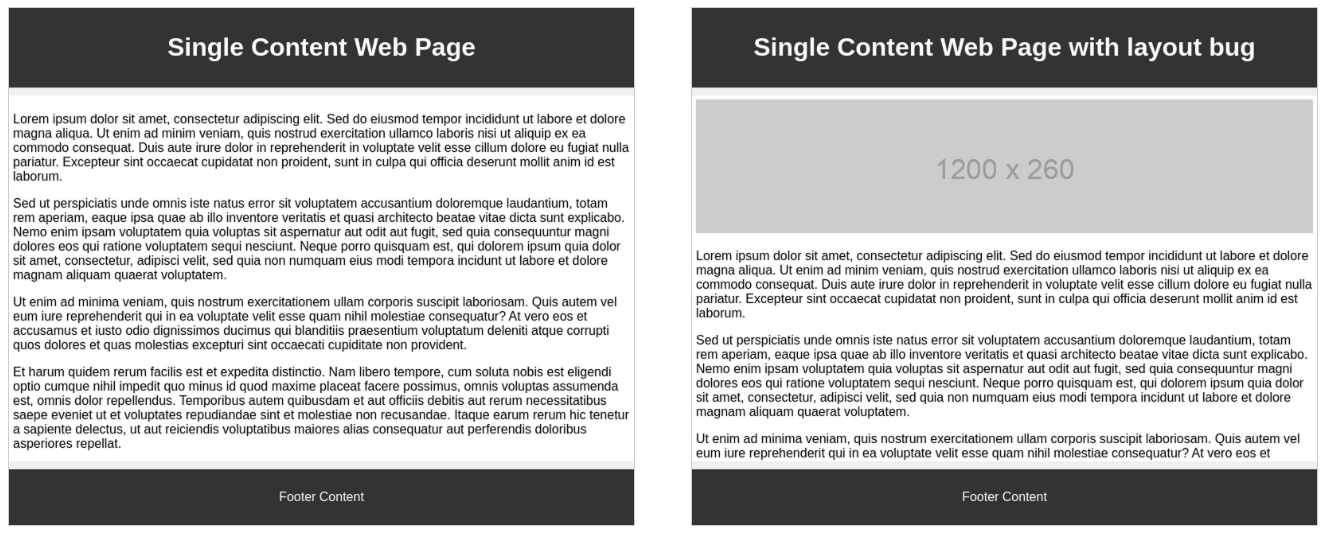
\includegraphics[width=1.0\columnwidth]{image/4_img_high_original_bf_af}
        \caption{「変更前高解像度画像」(左)と「変更後高解像度画像」(右)}
        \label{fig: high_img}
    \end{center}
\end{figure}
なお、生成した高解像度画像は他の処理部で使用するため、「変更前高解像度画像」と「変更後高解像度画像」をデータ管理部のdiff\_dirディレクトリに出力する。
\par
高解像度画像を生成する流れを、以下に示す。なお、リサイズに使用するリサンプリングフィルタには、LANCZOSフィルタ(\ref{sec:pillow}節を参照)を用いる。
\begin{enumerate}
    \item PillowのImage.open関数(\ref{sec:pillow}節を参照)にWebページの画像パスを渡して、base\_dirディレクトリから画像を読み込む。
    \item 画像の幅と高さを取得する。
    \item 画像の拡大率を設定する。本研究では、$2$とする。
    \item 画像のサイズ変更時に使用するリサンプリングフィルタを設定する。本研究では、PillowのImage.LANCZOSフィルタ(\ref{sec:pillow}節を参照)を用いる。
    \item Webページの画像を、画像の幅と高さそれぞれに画像の拡大率を掛けたサイズの高解像度画像にリサイズする。
\end{enumerate}


\subsection{適応的二値化処理}\label{subsec:Adaptive_Binarisation}
適応的二値化処理は、「変更前高解像度画像」と「変更後高解像度画像」のそれぞれに対して適応的二値化を行い、
「変更前高解像度二値化画像」と「変更後高解像度二値化画像」を生成する。
この処理により、画像の一部が明るく、他の部分が暗い場合においても、均一な二値化画像を生成できるため、
輪郭検出処理(\ref{subsec:contour_detection_processing}節で後述)の精度向上につながる。
図\ref{fig: high_img}に示した、「変更前高解像度画像」と「変更後高解像度画像」に適応的二値化処理を適用して生成した
「変更前高解像度二値化画像」と「変更後高解像度二値化画像」を、図\ref{fig: img_high_bin_bf_af}に示す。
\begin{figure}[tp]
    \begin{center}
        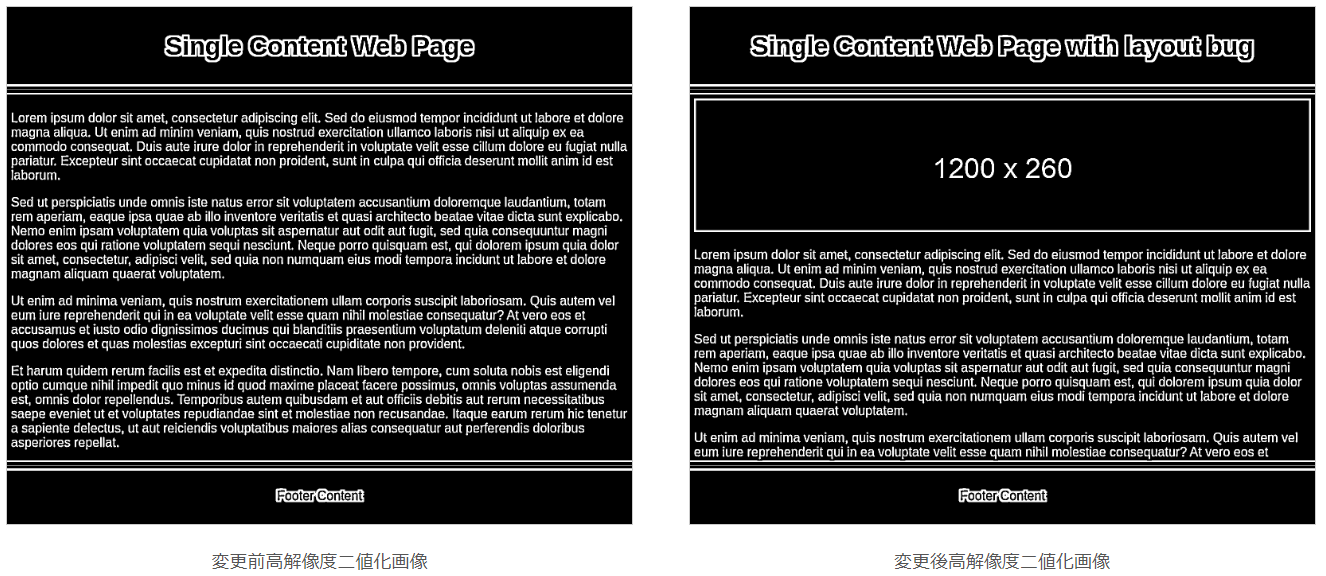
\includegraphics[width=1.0\columnwidth]{image/4_img_high_bin_bf_af.png}
        \caption{「変更前高解像度二値化画像」(左)と「変更後高解像度二値化画像」(右)}
        \label{fig: img_high_bin_bf_af}
    \end{center}
\end{figure}
\par
「変更前高解像度画像」と「変更後高解像度画像」に対して、それぞれ適応的二値化を行う流れを、以下に示す。
\begin{enumerate}
    \item imread関数(\ref{sec:opencv}節を参照)を用いて、変更前画像と変更後画像をそれぞれ読み込む。
    \item cvtColor関数(\ref{sec:opencv}節を参照)を用いて、変更前画像と変更後画像をそれぞれグレースケール化する。
    \item adaptiveThreshold関数(\ref{sec:opencv}節を参照)を用いて、2つのグレースケール画像に対して白黒反転を伴う適応的二値化をそれぞれ行う。
    \item 3.の処理結果により、「変更前高解像度二値化画像」と「変更後高解像度二値化画像」を生成する。
\end{enumerate}

\subsection{差分検出処理}\label{subsec:difference_detection_process}
差分検出処理は、「変更前高解像度二値化画像」と「変更後高解像度二値化画像」に対して、差分検出を行う。
処理の結果として、変更前画像から削除された箇所と、変更後画像に追加された箇所をそれぞれ白い部分として可視化した、
「削除箇所二値化画像」と「追加箇所二値化画像」を生成する。
図\ref{fig: img_high_bin_bf_af}に示した、「変更前高解像度二値化画像」と「変更後高解像度二値化画像」に
差分検出処理を適用して生成した「削除箇所二値化画像」と「追加箇所二値化画像」を、図\ref{fig: img_del_add_bin_bf_af}に示す。
\begin{figure}[tp]
    \begin{center}
        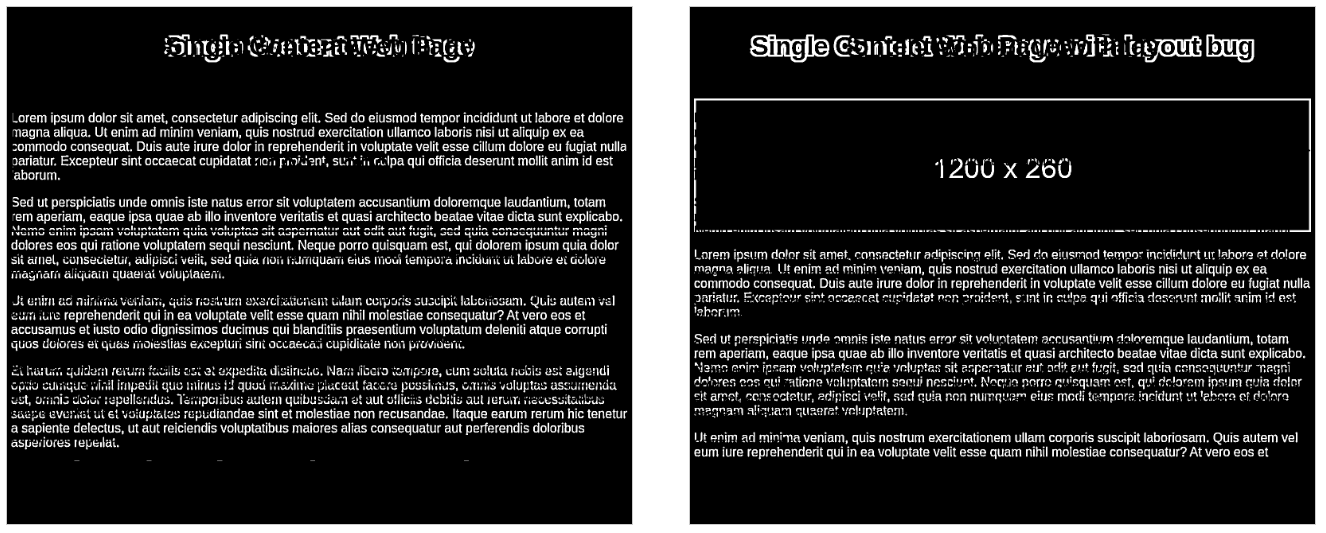
\includegraphics[width=1.0\columnwidth]{image/4_img_del_add_bin_bf_af.png}
        \caption{「削除箇所二値化画像」(左)と「追加箇所二値化画像」(右)}
        \label{fig: img_del_add_bin_bf_af}
    \end{center}
\end{figure}
図\ref{fig: img_del_add_bin_bf_af}を見ると、
図\ref{fig: img_high_bin_bf_af}の「変更前高解像度二値化画像」と「変更後高解像度二値化画像」を重ねたときの共通部分である白い箇所が消えており、
「変更前高解像度二値化画像」には、削除箇所が残り、「変更後高解像度二値化画像」には、追加箇所が残る。
これにより、輪郭検出処理(\ref{subsec:contour_detection_processing}節で後述)で、削除箇所を赤枠で、追加箇所を緑枠で囲むことができる。
\par
「変更前高解像度二値化画像」と「変更後高解像度二値化画像」に対して、差分検出処理を行う流れを、以下に示す。
\begin{enumerate}
    \item subtract関数(\ref{sec:opencv}節を参照)の第一引数に「変更前高解像度二値化画像」を指定し、
          第二引数に「変更後高解像度二値化画像」を指定する。
    \item 1のsubtract関数によって、変更前の画像には存在するが変更後の画像には存在しない箇所を可視化した「削除箇所二値化画像」を生成する。
    \item subtract関数(\ref{sec:opencv}節を参照)の第一引数に「変更後高解像度二値化画像」を指定し、
          第二引数に「変更前高解像度二値化画像」を指定する。
    \item 3のsubtract関数によって、変更後の画像には存在するが変更前の画像には存在しない箇所を可視化した「追加箇所二値化画像」を生成する。
\end{enumerate}

\subsection{膨張処理}\label{subsec:dilation}
% (\ref{sec:dilation}節を参照)
膨張処理は、「削除箇所二値化画像」と「追加箇所二値化画像」のそれぞれの白い部分の形状とサイズを強調する。
この処理により、削除箇所と追加箇所の輪郭検出処理(\ref{subsec:contour_detection_processing}節で後述)を高める。
処理の結果として、膨張処理を行った、「削除箇所強調二値化画像」と「追加箇所強調二値化画像」を生成する。
図\ref{fig: img_del_add_bin_bf_af}に示した、「削除箇所二値化画像」と「追加箇所二値化画像」に対して膨張処理を適用して生成した「削除箇所強調二値化画像」と「追加箇所強調二値化画像」を、図\ref{fig: img_del_add_highlight_bin}に示す。
\begin{figure}[tp]
    \begin{center}
        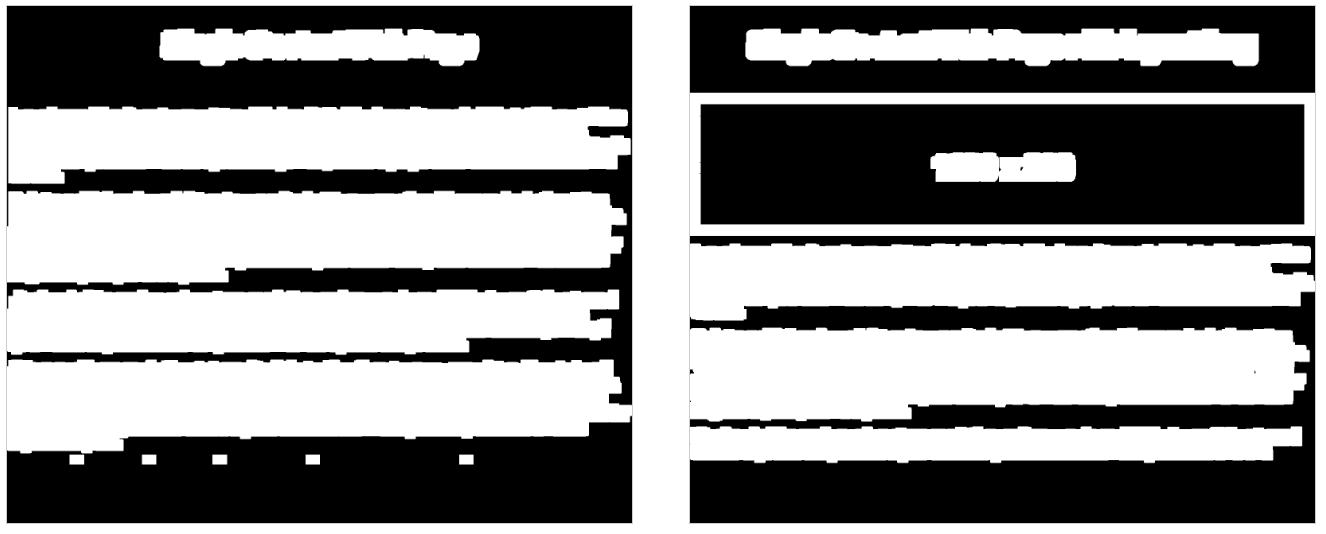
\includegraphics[width=1.0\columnwidth]{image/4_img_del_add_highlight_bin.png}
        \caption{「削除箇所強調二値化画像」(左)と「追加箇所強調二値化画像」(右)}
        \label{fig: img_del_add_highlight_bin}
    \end{center}
\end{figure}
\par
「削除箇所二値化画像」と「追加箇所二値化画像」に対して、膨張処理を適用する流れを、以下に示す。
\begin{enumerate}
    \item 特定の形状とサイズを持つカーネルを設定する。本研究では、5x5ピクセルの正方形カーネルを採用する。
    \item 設定したカーネルを用いて、膨張処理を適用する。適用後、画像内の削除箇所または追加箇所が拡大する。
    \item 2の膨張処理を複数回適用する。本研究では、膨張処理を6回繰り返すことで削除箇所または追加箇所を強調する。
    \item 膨張処理によって生成した「削除箇所強調二値化画像」と「追加箇所強調二値化画像」を輪郭検出処理に渡す。
\end{enumerate}

\subsection{輪郭検出処理}\label{subsec:contour_detection_processing}
輪郭検出処理は、findContours関数(\ref{sec:opencv}節を参照)を用いて「削除箇所強調二値化画像」と「追加箇所強調二値化画像」に対して、
削除箇所の輪郭と追加箇所の輪郭をそれぞれ検出する。
検出した輪郭は、輪郭リストとして格納しておく。
なお、検出した輪郭の面積が閾値未満の面積であれば、
検出した輪郭を輪郭リストに格納しない。
この処理は、閾値面積未満の輪郭を除外することによって、膨張処理で生じる可能性のあるノイズを除去し、
輪郭検出の精度を高めるために必要である。
この処理の結果として、輪郭の面積が閾値以上である、削除箇所の輪郭リストと追加箇所の輪郭リストを取得する。

\subsection{枠描画処理}\label{subsec:Bounding box drawing process}
枠描画処理は、変更前画像と変更後画像に対して輪郭検出処理(\ref{subsec:contour_detection_processing}節を参照)で取得した輪郭リストを用いて、
「差分箇所変更前画像」と「差分箇所変更後画像」を生成する。
また、それらの画像から枠のみを残してそれ以外の部分を黒くすることで、差分箇所を囲む色付きの枠のみを抽出した、
「差分箇所赤枠強調マスク画像」と「差分箇所緑枠強調マスク画像」を生成する。
「差分箇所変更前画像」と「差分箇所変更後画像」を、図\ref{fig: img_diff_highlight}に示す。
\begin{figure}[tp]
    \begin{center}
        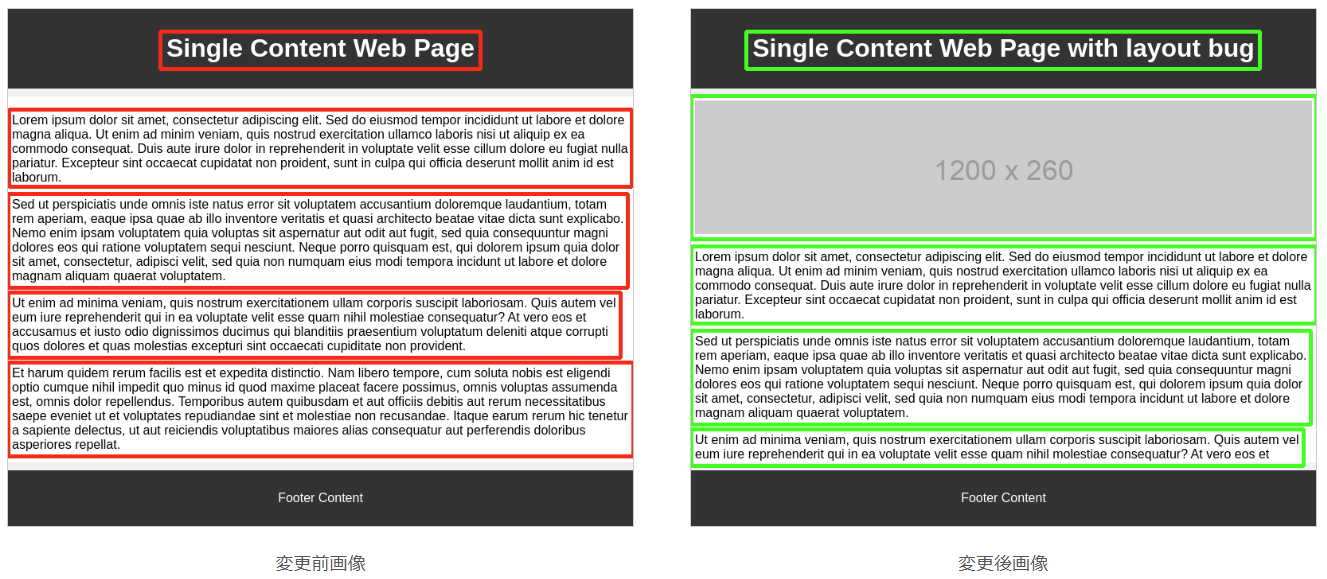
\includegraphics[width=1.0\columnwidth]{image/4_img_diff_highlight.png}
        \caption{「差分箇所変更前画像」(左)と「差分箇所変更後画像」(右)}
        \label{fig: img_diff_highlight}
    \end{center}
\end{figure}
また、「差分箇所赤枠強調マスク画像」と「差分箇所緑枠強調マスク画像」を、図\ref{fig: img_diff_highlight_mask}に示す。
\begin{figure}[tp]
    \begin{center}
        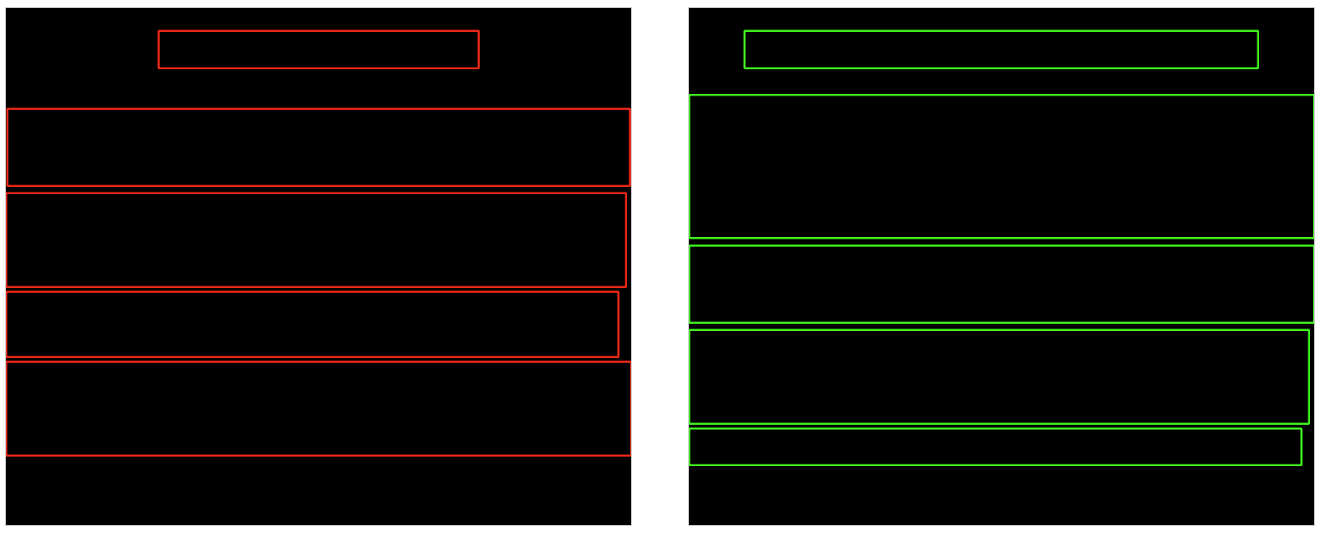
\includegraphics[width=1.0\columnwidth]{image/4_img_diff_highlight_mask.png}
        \caption{「差分箇所赤枠強調マスク画像」(左)と「差分箇所緑枠強調マスク画像」(右)}
        \label{fig: img_diff_highlight_mask}
    \end{center}
\end{figure}
\par
枠描画処理の流れを、以下に示す。
\begin{enumerate}
    \item boundingRect関数(\ref{sec:opencv}節を参照)を用いて、削除箇所の輪郭リストと追加箇所の輪郭リストのそれぞれの各要素である輪郭データから、輪郭を囲む矩形の座標と幅、高さを取得する。
    \item 取得した矩形情報を引数に指定したrectangle関数(\ref{sec:opencv}節を参照)を用いて、変更前画像上に赤枠、変更後画像上に緑枠を描画し、「差分箇所赤枠強調画像」と「差分箇所緑枠強調画像」をそれぞれ生成する。
    \item np.zeros関数(\ref{sec:numpy}節を参照)を用いて、変更前画像、または、変更後画像と同じサイズの2つの黒画像を生成する。
    \item 取得した矩形情報を引数に指定したrectangle関数を用いて、3.で生成した2つの黒画像に対して、
          一方の黒画像に赤枠のみを描画した「差分箇所赤枠強調マスク画像」、もう一方の黒画像に緑枠を描画した「差分箇所緑枠強調マスク画像」をそれぞれ生成する。
\end{enumerate}


%%%% HTML比較 %%%%
% 画像比較部は、データ管理部のbase\_dirディレクトリから変更前画像と変更後画像を受け取り、
% 画像比較に基づく差分箇所を色付きの枠で囲むことで強調表示した変更前画像と変更後画像を生成する。
% また、それらの画像から枠のみを残してそれ以外の部分を黒くすることで、差分箇所を囲む色付きの枠のみを抽出した、「差分箇所赤枠強調マスク画像」と「差分箇所緑枠強調マスク画像」も生成する。
% 生成した画像は、データ管理部のbase\_dirディレクトリに出力する。
% \par
% 画像比較部の処理の流れを、以下に示す。
% \begin{enumerate}
%     \item 高解像度画像生成処理
%     \item 適応的二値化処理
%     \item 差分検出処理
%     \item 膨張処理
%     \item 輪郭検出処理
%     \item 枠描画処理
% \end{enumerate}
% また、\toolName の入力対象とする変更前画像と変更後画像の例を、図\ref{fig: img_original_bf_af}に示す。
% \begin{figure}[tp]
%     \begin{center}
%         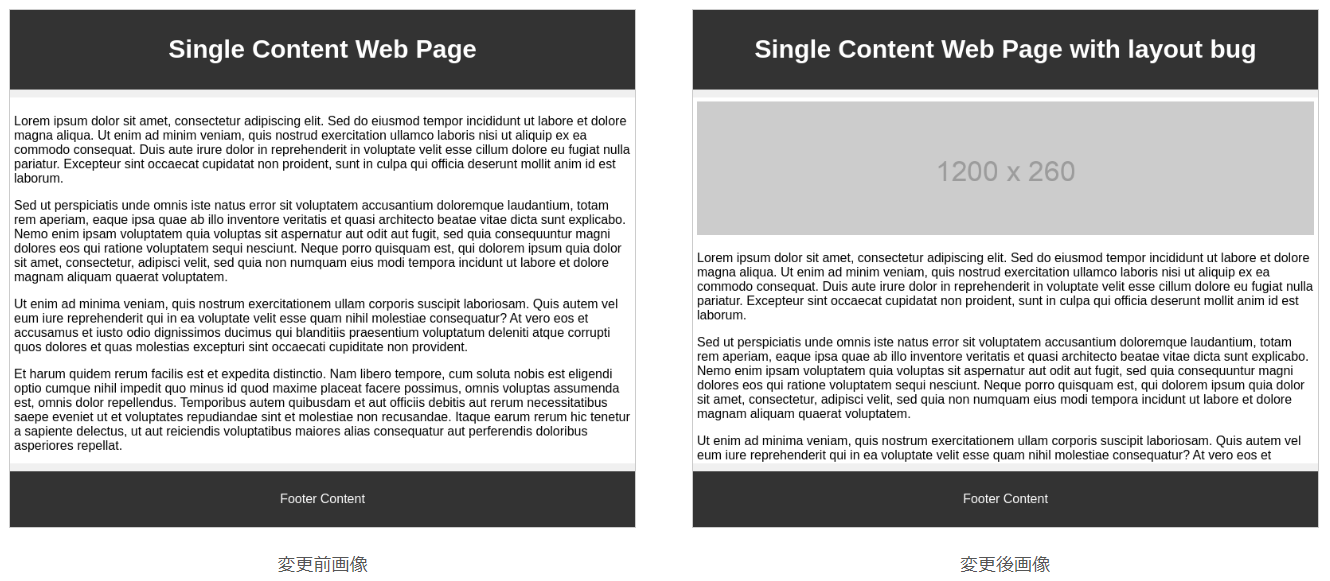
\includegraphics[width=1.0\columnwidth]{image/4_img_original_bf_af.png}
%         \caption{\toolName の入力対象とする変更前画像と変更後画像の例}
%         \label{fig: img_original_bf_af}
%     \end{center}
% \end{figure}
% 以降、具体例に図\ref{fig: img_original_bf_af}を用いて、画像比較部の各処理について説明する。
\section{HTML比較部}\label{sec:Affected_area_extraction}
HTML比較部は、データ管理部のbase\_dirディレクトリ(表\ref{tb: base_dir_data}を参照)から変更前HTMLコードと変更後HTMLコードを受け取り、
「変更箇所変更前画像」と「変更箇所変更後画像」を生成する。
また、それらの画像から枠のみを残してそれ以外の部分を黒くすることで、変更箇所を囲む色付きの枠のみを抽出した、「変更箇所赤枠強調マスク画像」と「変更箇所緑枠強調マスク画像」を生成する。
\par
HTML比較部の処理の流れを、以下に示す。
\begin{enumerate}
    \item 差分コード生成処理
    \item 枠付きHTMLコード生成処理
    \item 枠抽出処理
\end{enumerate}
\par
以降、HTML比較部の各処理について説明する。
% 以降、図\ref{fig: img_original_bf_af}の例で挙げたWebページの、変更前HTMLコードと変更後HTMLコードを具体例に、
% HTML比較部の各処理について説明する。

\subsection{差分コード生成処理}\label{subsec:diff_file_generate}
差分コード生成処理は、Webページの変更前HTMLコードと変更後HTMLコードを行ごとに比較して、txt形式の差分コードを生成する。
生成したtxt形式の差分コードの例を、ソースコード\ref{lst:diff_html}に示す。
ソースコード\ref{lst:diff_html}の3行目を見ると、先頭に"-"が付いており、この行は削除された行であることを示す。
また、ソースコード\ref{lst:diff_html}の4行目および8行目を見ると、先頭に"+"が付いており、この行は追加された行であることを示す。
このように、生成したtxt形式の差分コードには、コードの追加された行の先頭に"+"、削除された行の先頭に"-"を付加する。
\begin{figure}[tp]
    \begin{lstlisting}[language=HTML, caption=生成したtxt形式の差分コードの例, label=lst:diff_html]
<body>
    <header>
-         <h1>Single Content Web Page</h1>
+         <h1>Single Content Web Page with layout bug</h1>
    </header>
    <div class="container">
        <div class="main-content">
+             <img src="https://via.placeholder.com/1200x260" alt="Placeholder Image">
              // テキスト文省略
        </div>
    </div>
    <footer>
        <p>Footer Content</p>
    </footer>
</body>
    \end{lstlisting}
\end{figure}
\par
差分コードを生成する処理を、以下に示す。
\begin{enumerate}
    \item 変更前HTMLコードと変更後HTMLコードをそれぞれHTMLデータとして読み込む。
    \item HTMLデータ内の$<$p$>$タグ内のテキスト内に存在する余分な空白や改行を取り除くために、以下を行う。
          \begin{enumerate}
              \item 変更前と変更後のHTMLデータを解析するためのBeautifulSoupオブジェクト(\ref{sec:beautifulsoup}節を参照)をそれぞれ初期化する。
              \item BeautifulSoupオブジェクトに対して、find\_all関数(\ref{sec:beautifulsoup}節を参照)を用い、HTMLデータ内の全ての$<$p$>$タグを格納したリストを生成する。
              \item get\_text関数(\ref{sec:beautifulsoup}節を参照)を用いて、生成したリストの各要素内における$<$p$>$タグのテキストを取得する。
              \item Pythonの文字列関数であるsplit関数を用いて、タブや改行などの連続する空白を1つの区切りとみなし、テキストを単語ごとに分割する。
              \item Pythonの文字列関数であるjoin関数を用いて、分割された単語を1つの空白のみで結合する。
              \item BeautifulSoupオブジェクトをstring型に変換し、HTMLデータ形式に戻す。
          \end{enumerate}
    \item difflib(\ref{sec:difflib}節を参照)のDifferクラスのcompareメソッドを用いて、2つのHTMLデータ間を行ごとに比較し、差分コードを生成する。
    \item 生成した差分コードから、行の先頭が"?"から始まる行を除外する。
          これは、本研究では、"?"で始まる行については、解析の対象としないためである。
    \item 差分コードをtxt形式で保存する。
\end{enumerate}

% \subsection{差分コード解析処理}\label{subsec:diff_file_analyze}
% 差分コード解析処理は、差分コード生成処理から差分コードを受け取り、差分コードからbody要素内の変更箇所とstyle要素内の変更箇所を検出する。
% \par
% 差分コードを解析する処理を、以下に示す。

% 枠付きHTMLコード生成するためには、以下の処理を行う。
% body要素内の変更箇所を検出する。
% 差分コードの先頭の行に対して、以下の処理を行う。
% 1.body要素外であるか判定する。body要素外ならば、以下の処理を行う。
% 1. 先頭行が"-"であれば、
% body要素内の各先頭行に"+"または"-"がある箇所を探す。
% "+"や"-"であれば、その行に対して以下の操作を行う。
% 1."+"または"-"を削除する。
% 2.行にimgタグが含まれている場合、img用の枠を囲むCSSクラスを追加する。
% 3.行にimgタグが含まれていない場合、行中に開始タグが存在するかを確認する。
% 4.行中に開始タグが存在する場合は、タグ内にclass属性が既にあるかどうか確認する。行中に開始タグが存在しない場合は、何もしない。
% 5.class属性があれば、class=""の中の末尾に枠をつけるクラスを追加する。
% 6.class属性が無ければ、終了タグ直前に枠をつけるクラスを追加する。

% body要素内の変更箇所に枠をつけるCSSクラスを追加する。
% style要素内の変更箇所を検出する。
% style要素内の変更箇所に枠をつけるCSSクラスを追加する。

\subsection{枠付きHTMLコード生成処理}\label{subsec:modified_html_generate}
枠付きHTMLコード生成処理は、差分コード生成処理から差分コードを受け取り、
枠付き変更前HTMLコードと枠付き変更後HTMLコードを生成する。
生成した枠付き変更前HTMLコードと枠付き変更後HTMLコードは、データ管理部のdiff\_dirディレクトリ(\ref{tb: diff_dir_data}節を参照)に出力する。
\par
差分コードから、枠付き変更前HTMLコードと枠付き変更後HTMLコードを生成する処理を、以下に示す。
\begin{enumerate}
    \item body要素解析処理
    \item CSSセレクタ抽出処理
    \item CSSクラス付加処理
\end{enumerate}

\subsubsection{body要素解析処理}\label{subsubsec: body_analysis}
body要素解析処理は、差分コード生成処理から受け取った差分コードにおいて、
body要素内で変更があったタグ要素のstyle属性にCSSクラス\cite{CssSelector}を付加した、変更前HTMLコードを格納するリストmodified\_before\_linesと
変更後HTMLコードを格納するリストmodified\_after\_linesを生成し、後述するCSSクラス付加処理に出力する。
\par
body要素解析処理の流れを、以下に示す。
なお、modified\_before\_linesとmodified\_after\_linesを、それぞれ空リストとして初期化する。
また、現在処理中の行において、削除された行であるかどうかを示す変数flag\_beforeの値と、追加された行であるかどうかを示す変数flag\_afterの値を、それぞれFalseで初期化する。
さらに、差分コードの全ての行に対して、先頭行から順に1行ずつ、以下の処理を行う。
\begin{enumerate}
    \item 行がbody要素外の場合:
          \begin{itemize}
              \item 行の先頭が“-”の場合、modified\_before\_linesに行を追加する。
              \item 行の先頭が“+”の場合、modified\_after\_linesに行を追加する。
              \item 行の先頭がそれ以外の場合、modified\_before\_linesとmodified\_after\_linesの両方に行を追加する。
          \end{itemize}
    \item 行がbody要素内の場合:
          \begin{enumerate}
              \item 行の先頭を調べて、以下の処理を行う。
                    \begin{itemize}
                        \item 行の先頭が“-”、または、“+”以外の場合、
                              flag\_beforeの値とflag\_afterの値をともにFalseにする。
                        \item 行の先頭が“-”の場合、flag\_beforeの値をTrueにする。
                        \item 行の先頭が“+”の場合、flag\_afterの値をTrueにする。
                    \end{itemize}
              \item 行中に“\textless img”を含むかどうかを調べて、以下の処理を行う。
                    \begin{itemize}
                        \item 行中に“\textless img”を含む場合は、imgタグ用のCSSクラス(\ref{subsubsec: css_define}節に後述)を付加したdivタグでimgタグを囲む。
                        \item 行中に“\textless img”を含まない場合は、以下のどちらかの処理を行う。
                              \begin{itemize}
                                  \item 行中に“class=”を含む場合、開始タグのstyle属性にbody要素用のCSSクラス(\ref{subsubsec: css_define}節に後述)を付加する。
                                  \item 行中に“class=”を含まない場合、開始タグの終了記号直前にbody要素用のCSSクラスを付加する。
                              \end{itemize}
                    \end{itemize}
              \item flag\_beforeの値とflag\_afterの値を調べて、以下の処理を行う。
                    \begin{itemize}
                        \item flag\_beforeの値がTrue、かつ、flag\_afterの値がFalseの場合、modified\_before\_linesに行を追加する。
                        \item flag\_beforeの値がFalse、かつ、flag\_afterの値がTrueの場合、modified\_after\_linesに行を追加する。
                        \item flag\_beforeの値とflag\_afterの値がそれ以外の場合、modified\_before\_linesとmodified\_after\_linesの両方に行を追加する。
                    \end{itemize}
          \end{enumerate}
    \item modified\_before\_linesとmodified\_after\_linesを、後述するCSSクラス付加処理に出力する。
\end{enumerate}

\subsubsection{CSSセレクタ抽出処理}\label{subsubsec: style_analysis}
CSSセレクタ抽出処理は、差分コード生成処理から受け取った差分コードにおいて、style要素内で変更があったCSSセレクタ\cite{CssSelector}を、差分コードから全て抽出する。
抽出したCSSセレクタは、リストにそれぞれ格納し、後述するCSSクラス付加処理に出力する。
\par
CSSセレクタ抽出処理の流れを、以下に示す。
\begin{enumerate}
    \item 変更があったCSSセレクタを格納するリストであるchanged\_selectorsを、空リストとして初期化する。
    \item 現在処理中のCSSセレクタを保持するための変数であるcurrent\_selectorの値を、Noneに初期化する。
    \item 差分コードの全ての行に対して、先頭行から順に1行ずつ文字列の判定をし、判定結果に応じて、以下の処理を行う。
          \begin{itemize}
              \item CSSセレクタの開始を示す“\{”を含む行を見つけた場合:
                    \begin{enumerate}
                        \item 行中のCSSセレクタのみを抽出する。
                        \item changed\_selectors内に抽出したセレクタが存在せず、かつ、行が変更を示す“+”、または、“-”で始まる場合、
                              CSSセレクタをchanged\_selectorsに格納する。
                        \item current\_selectorの値にCSSセレクタを格納し、現在処理中のCSSセレクタを更新する。
                    \end{enumerate}
              \item current\_selectorの値にCSSセレクタが格納されており、行が変更を示す"+"、または、"-"で始まる場合:
                    \begin{itemize}
                        \item changed\_selectors内に、current\_selectorに格納されているCSSセレクタが存在しないならば、
                              そのCSSセレクタをchanged\_selectorsに格納する。
                    \end{itemize}
              \item CSSセレクタの終了を示す“\}”を含む行を見つけた場合:
                    \begin{itemize}
                        \item current\_selectorの値にNoneを格納し、現在処理中のCSSセレクタをリセットする。
                    \end{itemize}
          \end{itemize}
    \item changed\_selectorsを、後述するCSSクラス付加処理に出力する。
\end{enumerate}

\subsubsection{CSSクラス付加処理}\label{subsubsec: css_define}
CSSクラス付加処理は、body要素内で変更があったタグ要素のstyle属性にCSSクラス\cite{CssSelector}を付加した変更前HTMLコードのstyle要素の末尾に、
変更箇所における削除箇所に赤枠をつけるCSSクラスを付加し、枠付き変更前HTMLコードを生成する。
また、body要素内で変更があったタグ要素のstyle属性にCSSクラスを付加した変更後HTMLコードのstyle要素の末尾に、
変更箇所における追加箇所に緑枠をつけるCSSクラスを付加し、枠付き変更後HTMLコードを生成する。
\par
変更箇所に色枠をつける6種類のCSSクラスを、以下に定義する。
\begin{itemize}
    \setlength{\itemsep}{0pt}
          \setlength{\parsep}{0pt}
    \item UNIQUE\_CLASS\_BEFORE\_CSS:\\
          body要素内での削除、または変更があった画面要素を赤枠で囲むスタイルを定義したCSSクラス。
    \item UNIQUE\_CLASS\_AFTER\_CSS:\\
          body要素内での追加、または変更があった画面要素を緑枠で囲むスタイルを定義したCSSクラス。
    \item IMAGE\_WRAPPER\_CLASS\_BEFORE\_CSS:\\
          body要素内での削除、または、CSSの変更があった画像を赤枠で囲むスタイルを定義したCSSクラス。
    \item IMAGE\_WRAPPER\_CLASS\_AFTER\_CSS:\\
          body要素内での追加、または、CSSの変更があった画像を緑枠で囲むスタイルを定義したCSSクラス。
    \item SELECTORS\_CLASS\_BEFORE\_CSS:\\
          style要素内で変更があった、1つ以上のCSSセレクタに赤枠を付加するスタイルを定義したCSSクラス。
    \item SELECTORS\_CLASS\_AFTER\_CSS:\\
          style要素内で変更があった、1つ以上のCSSセレクタに緑枠を付加するスタイルを定義したCSSクラス。
\end{itemize}
\par
CSSクラス付加処理の流れを、以下に示す。
\begin{enumerate}
    \item body要素解析処理から、modified\_before\_linesと、modified\_after\_linesを受け取る。
    \item CSSセレクタ抽出処理から、変更があったCSSセレクタを格納するリストchanged\_selectorsを受け取る。
    \item 枠付き変更前HTMLコードを格納するリストfinal\_before\_linesと、枠付き変更後HTMLコードを格納するリストfinal\_after\_linesを空リストとして初期化する。
    \item modified\_before\_lines内の先頭行から順に、各行に対して、以下の処理を行う。
          \begin{itemize}
              \item "$<$/style$>$"を含まない行の場合、final\_before\_linesに行を追加する。
              \item "$<$/style$>$"を含む行を見つけた場合は、以下の処理を行う。
                    \begin{enumerate}
                        \item final\_before\_linesに、UNIQUE\_CLASS\_BEFORE\_CSSと\\IMAGE\_WRAPPER\_CLASS\_BEFORE\_CSSを追加する。
                        \item changed\_selectorsの要素数が$0$より大きい場合、final\_before\_linesに、\\SELECTORS\_CLASS\_BEFORE\_CSSを追加する。
                        \item final\_before\_linesに、"$<$/style$>$"を含む行を加える。
                    \end{enumerate}
          \end{itemize}
    \item modified\_after\_lines内の先頭行から順に、各行に対して、以下の処理を行う。
          \begin{itemize}
              \item "$<$/style$>$"を含まない行の場合、final\_after\_linesに行を追加する。
              \item "$<$/style$>$"を含む行を見つけた場合は、以下の処理を行う。
                    \begin{enumerate}
                        \item final\_after\_linesに、UNIQUE\_CLASS\_AFTER\_CSSと\\IMAGE\_WRAPPER\_CLASS\_AFTER\_CSSを追加する。
                        \item changed\_selectorsの要素数が$0$より大きい場合、final\_after\_linesに、\\SELECTORS\_CLASS\_AFTER\_CSSを追加する。
                        \item final\_after\_linesに、"$<$/style$>$"を含む行を加える。
                    \end{enumerate}
          \end{itemize}
    \item final\_before\_linesをHTMLコード形式で保存し、枠付き変更前HTMLコードを生成する。
    \item final\_after\_linesをHTMLコード形式で保存し、枠付き変更後HTMLコードを生成する。
\end{enumerate}
% style要素内の末尾に、body要素内で変更があった、画像以外のタグ要素にCSSクラスを付加する。なお、画像の追加や削除、変更があれば、imgタグ用のCSSクラスを付加する。
% また、CSSセレクタ抽出処理から受け取った、変更があったCSSセレクタを格納するリストchanged\_selectorsに、1つ以上のCSSセレクタを含む場合は、
% CSSセレクタ用のCSSクラスをstyle要素内の末尾に付加する。

\subsection{枠抽出処理}\label{subsec:frame_extraction}
枠抽出処理は、
変更前画像と「枠付き変更前画像」を比較し、赤枠のみを抽出した「変更箇所赤枠強調マスク画像」を生成する。
また、変更後画像と「枠付き変更後画像」を比較し、緑枠のみを抽出した「変更箇所緑枠強調マスク画像」を生成する。
「変更箇所変更前後画像」を、図\ref{fig: html_waku}に示す。
なお、「枠付き変更前画像」と「枠付き変更後画像」の2つの画像を総称して、「変更箇所変更前後画像」と呼ぶ。
\begin{figure}[tp]
    \begin{center}
        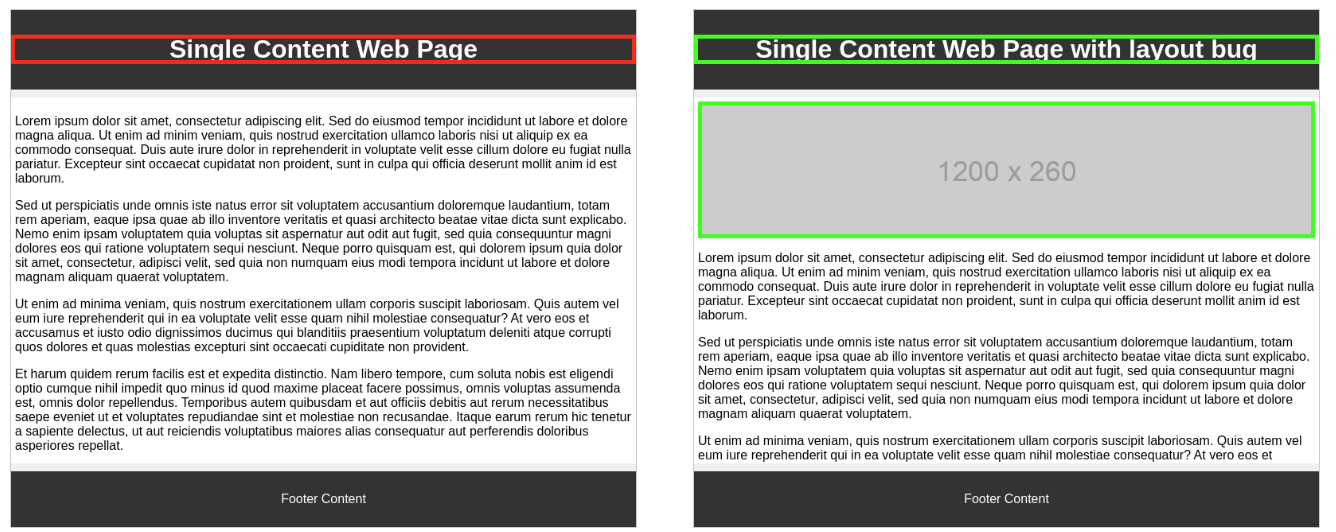
\includegraphics[width=1.0\columnwidth]{image/4_html_waku.png}
        \caption{「変更箇所変更前画像」(左)と「変更箇所変更後画像」(右)}
        \label{fig: html_waku}
    \end{center}
\end{figure}
また、「変更箇所赤枠強調マスク画像」と「変更箇所緑枠強調マスク画像」を、図\ref{fig: html_diff_mask}に示す。
\begin{figure}[tp]
    \begin{center}
        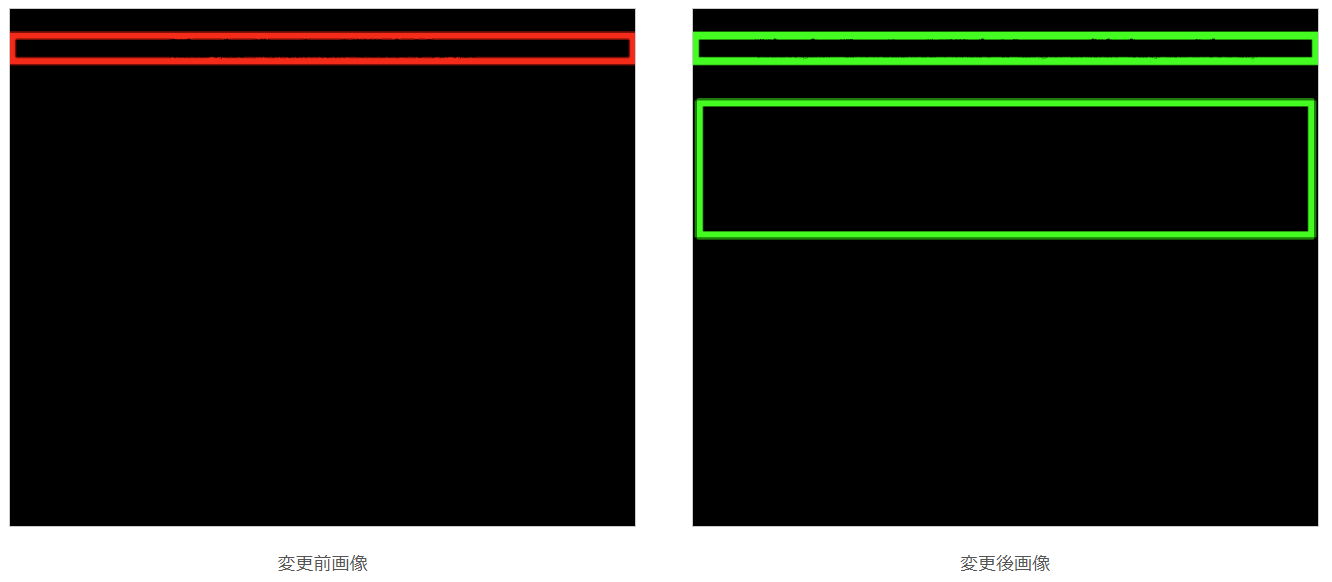
\includegraphics[width=1.0\columnwidth]{image/4_html_diff_mask.png}
        \caption{「変更箇所赤枠強調マスク画像」(左)と「変更箇所緑枠強調マスク画像」(右)}
        \label{fig: html_diff_mask}
    \end{center}
\end{figure}
\par
枠抽出処理の流れを、以下に示す。
\begin{enumerate}
    \item データ管理部のbase\_dirディレクトリから、変更前画像と変更後画像を受け取る。
    \item データ管理部のdiff\_dirディレクトリから、枠付き変更前HTMLコードと枠付き変更後HTMLコードを受け取る。
    \item 枠付き変更前HTMLコードと枠付き変更後HTMLコードを、ローカルサーバ上(\ref{sec:Flask}節を参照)で、それぞれWebページとして公開する。
    \item 3で公開したそれぞれのWebページのURLを、取得部に渡す。これにより、取得部は、
          枠付き変更前画像と枠付き変更後画像を取得し、取得した2つの画像を、データ管理部のdiff\_dirディレクトリに出力する。
    \item データ管理部のdiff\_dirディレクトリから、枠付き変更前画像と枠付き変更後画像を取得する。
    \item absdiff関数を用いて、変更前画像と枠付き変更前画像を比較し、「変更箇所赤枠強調マスク画像」を生成する。
    \item absdiff関数を用いて、変更後画像と枠付き変更後画像を比較し、「変更箇所緑枠強調マスク画像」を生成する。
\end{enumerate}

% \section{変更箇所検出部}\label{sec:Affected_area_extraction}
% HTMLコードの変更に基づく変更箇所抽出部は、Webページ情報取得部で取得した変更前後のWebページのHTMLコードを用いて変更箇所を特定する。
% 概要としては、差分コードを生成し、差分コードから枠付き処理を行った変更前後のHTMLコードを生成した後、そのHTMLコードをFlaskのテンプレートエンジンを用いてWebページを表示し、Webページ情報取得部によってそのWebページの画像を取得する。
% 元のWebページ画像と枠付き処理をしたWebページ画像を比較して枠のみを抽出する。
% 具体的には、まず、Pythonライブラリの一つであるdifflibモジュールを用いて、変更前後のHTMLコードから差分コードを生成する。
% 生成した差分コードは、コードの追加行には"+", 削除行には"-", 変更前後のHTMLコードにどちらにも存在しない行には"?"が先頭に付き、"?"を除いた差分コードを解析対象とする。
% 差分コードは、bodyタグ内とstyleタグ内を対象とする。
% もし、bodyタグ内で先頭に"+"や"-"があれば、コードの追加や削除、変更があったとして、その箇所に枠付き処理を行うCSSクラスを追加し、先頭の"+"か"-"を削除する。
% styleタグ内の場合は、CSSクラスのセレクタ名のみの変更やスタイルのみの変更、またはその両方の変更があったCSSクラスを対象として、そのCSSクラスに対して枠付きを行うスタイルを適用する。
% この場合においても、解析した行の先頭に"+", "-"があれば削除する。
% 差分コードから枠付き処理を行った変更前後のHTMLコードを生成した後は、そのHTMLコードをFlaskのテンプレートエンジンを用いてWebページとして表示し、そのWebページの画像を取得する。
% そして、元のWebページ画像と枠付き処理をしたWebページ画像を比較して枠のみを抽出する。
\section{不具合検出部}\label{sec:Layout_bug_extraction_section}
不具合検出部は、データ管理部のbase\_dirディレクトリから「変更前画像」と「変更後画像」を受け取り、また、
データ管理部のdiff\_dirディレクトリから「差分箇所赤枠強調マスク画像」と「差分箇所緑枠強調マスク画像」、「変更箇所赤枠強調マスク画像」と「変更箇所緑枠強調マスク画像」
をそれぞれ受け取ることで、「不具合箇所変更前画像」と「不具合箇所変更後画像」を生成する。
「不具合箇所変更前画像」と「不具合箇所変更後画像」を、図\ref{fig: 4_subeffect}に示す。
\begin{figure}[tp]
    \begin{center}
        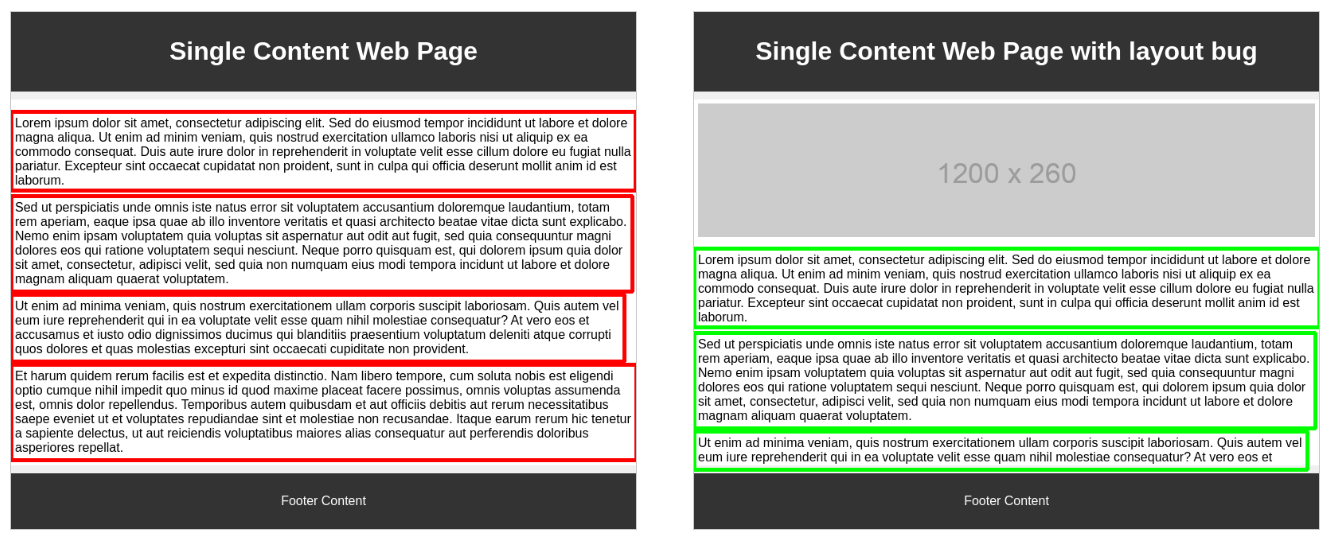
\includegraphics[width=1.0\columnwidth]{image/4_subEffect.png}
        \caption{「不具合箇所変更前画像」(左)と「不具合箇所変更後画像」(右)}
        \label{fig: 4_subeffect}
    \end{center}
\end{figure}
\par
% なお、レイアウトの不具合箇所を、赤枠で囲むことで強調表示した、変更前画像を「不具合箇所赤枠強調画像」、
% レイアウトの不具合箇所を、緑枠で囲むことで強調表示した、変更後画像を「不具合箇所緑枠強調画像」と定義する。
\par
不具合検出部の処理の流れを、以下に示す。
「差分箇所赤枠強調マスク画像」と「変更箇所赤枠強調マスク画像」を比較することで、
「差分箇所赤枠強調マスク画像」に存在する赤枠の中から、レイアウトの不具合箇所によって生じた赤枠の輪郭座標のみを抽出する。
また、「差分箇所緑枠強調マスク画像」と「変更箇所緑枠強調マスク画像」を比較することで、
「差分箇所緑枠強調マスク画像」に存在する緑枠の中から、レイアウトの不具合箇所によって生じた緑枠の輪郭座標のみを抽出する。
なお、二値化した「差分箇所赤枠強調マスク画像」からレイアウトの不具合箇所によって生じた赤枠の輪郭座標のみを格納するリストをunique\_contours\_bf、
レイアウトの不具合箇所によって生じた緑枠の輪郭座標のみを格納するリストをunique\_contours\_afとする。
\begin{enumerate}
    \item 「差分箇所赤枠強調マスク画像」と「変更箇所赤枠強調マスク画像」をimread関数(\ref{sec:opencv}節を参照)を用いて、読み込む。
    \item cvtColor関数(\ref{sec:opencv}節を参照)を用いて、グレースケール化する。
    \item threshold関数(\ref{sec:opencv}節を参照)を用いて、グレースケール画像に対して白黒反転を伴う二値化を行う。
    \item 二値化した「差分箇所赤枠強調マスク画像」に対して、findContours関数(\ref{sec:opencv}節を参照)を用いて、赤枠の輪郭リストを格納するリストcontours\_img\_bfを取得する。
    \item 二値化した「変更箇所赤枠強調マスク画像」に対して、findContours関数を用いて、緑枠の輪郭リストを格納するリストcontours\_html\_bfを取得する。
    \item contours\_img\_bfの各輪郭要素の数だけループして、以下の処理を行う。
          \begin{enumerate}
              \item contours\_html\_bfの各輪郭要素の数だけループして、以下の処理を行う。
                    \begin{enumerate}
                        \item contours\_img\_bfとcontours\_html\_bfのそれぞれの輪郭要素のバウンディングボックスを、boundingRect関数(\ref{sec:opencv}節を参照)を用いて取得する。
                        \item 2つのバウンディングボックスが対応するかどうかを示す変数matchの値をFalseに設定する。
                        \item バウンディングボックスが重なっているかどうかを判定する
                              \begin{itemize}
                                  \item  重なっている場合は、重なり部分のバウンディングボックスの面積を計算する。
                                        小さい方のバウンディングボックスの面積を計算し、
                                        バウンディングボックスの重なり部分の面積が、小さい方のバウンディングボックスの面積の5割を超えれば、
                                        大きい方のバウンディングボックスと小さい方のバウンディングボックスが対応すると判定し、Trueを返す。そうでなければ、Falseを返す。
                                  \item 対応しない場合は、Falseを返す。
                              \end{itemize}
                        \item matchの値がTrueの場合は、ループ処理から抜ける。
                    \end{enumerate}
              \item matchの値がTrueの場合に、contours\_img\_bfのうち、どのcontours\_html\_bfの輪郭要素とも重ならなかった輪郭要素を、unique\_contours\_bfに格納する。
          \end{enumerate}
    \item 「差分箇所緑枠強調マスク画像」と「変更箇所緑枠強調マスク画像」に対しても、同様に1.~6.の操作を行い、
          matchの値がTrueの場合、contours\_img\_afのうち、どのcontours\_html\_afの輪郭要素とも重ならなかった輪郭要素を、unique\_contours\_afに格納する。
    \item boundingRect関数を用いて、unique\_contours\_bfとunique\_contours\_afのそれぞれの輪郭リストの各要素である輪郭データから、輪郭を囲む矩形の座標と幅、高さを、矩形情報として取得する。
    \item 取得した矩形情報を引数に指定したrectangle関数を用いて、変更前画像上に赤枠、変更後画像上に緑枠を描画し、「不具合箇所変更前画像」と「不具合箇所変更後画像」を生成する。
\end{enumerate}

% \subsection{不具合抽出処理}\label{subsec:Layout_bug_extraction}
% 不具合抽出処理は、副作用抽出処理から、レイアウトの副作用によって生じた赤枠の輪郭座標のみを格納するリストunique\_contours\_bfと、
% レイアウトの副作用によって生じた緑枠の輪郭座標のみを格納するリストunique\_contours\_afを受け取り、
% レイアウトの副作用箇所からレイアウトの不具合箇所のみを抽出する。
% 抽出後、図\ref{fig: img_bug}に示した、
% レイアウトの不具合箇所を、色付きの枠で囲むことで強調表示した、変更前画像と変更後画像を生成する。
% \par
% \begin{figure}[tp]
%     \begin{center}
%         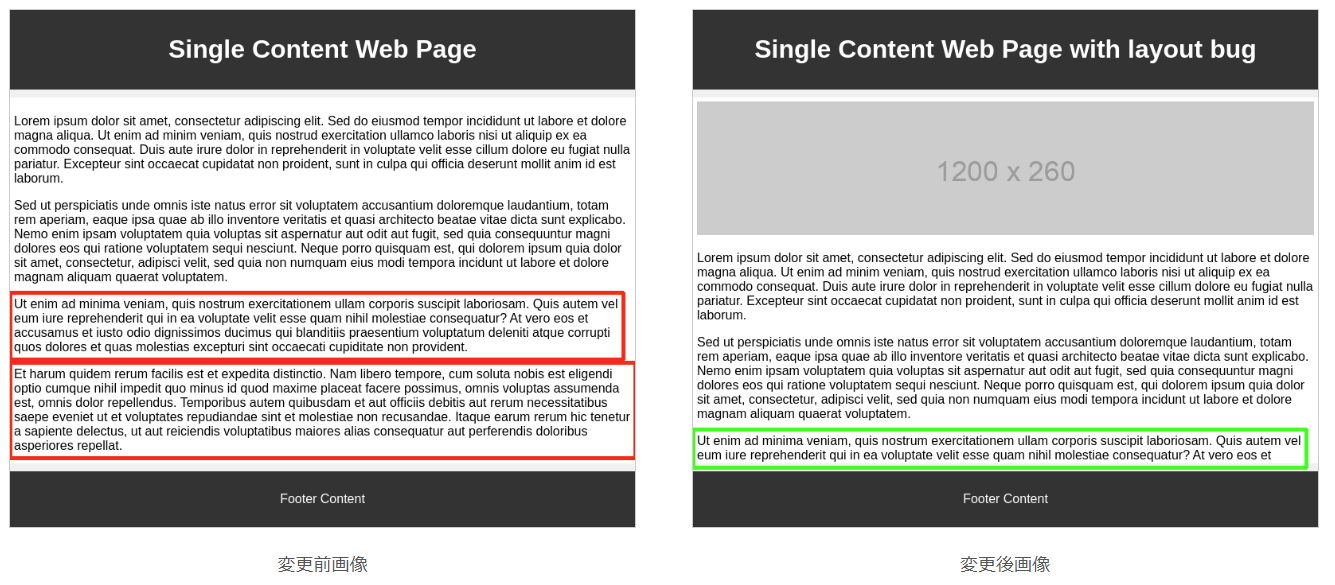
\includegraphics[width=1.0\columnwidth]{image/4_img_buf.png}
%         \caption{レイアウトの不具合箇所を、色付きの枠で囲むことで強調表示した、変更前画像と変更後画像}
%         \label{fig: img_bug}
%     \end{center}
% \end{figure}
% \par
% 不具合抽出処理を、以下に示す。
% \begin{enumerate}
%     \item unique\_contours\_bfの各輪郭要素の数だけループして、以下の処理を行う。
%           \begin{enumerate}
%               \item unique\_contours\_afの各輪郭要素の数だけループして、以下の処理を行う。
%                     \begin{enumerate}
%                         % \item unique\_contours\_bfの輪郭に対するバウンディングボックスの座標とサイズを計算し、
%                         %       そのバウンディングボックスに基づいて変更前画像から特定の領域を切り出す。
%                         % \item unique\_contours\_afの輪郭に対するバウンディングボックスの座標とサイズを計算し、
%                         %       そのバウンディングボックスに基づいて変更後画像から特定の領域を切り出す。
%                         \item unique\_contours\_bfとunique\_contours\_afのそれぞれの輪郭要���のバウンディングボックスを、boundingRect関数を用いて取得する。
%                         \item unique\_contours\_bfで取得したバウンディングボックスの座標とサイズに基づき、「変更前高解像���画像������対応する画像領域region\_bfを抽出する。
%                         \item unique\_contours\_afで取得したバウンディングボ�����クスの座標とサイズに基づき、「�����更後高解像度画像」から対応する画像領域region\_afを抽出する。
%                         \item absdiff関数を用いて、region\_bfとregion\_afの画像領域間の各ピクセル値の絶対値の差を計算し、類似度を求める。
%                         \item 類似度が9.5割を超えれば、レイアウトの不具合は無いと判定し、unique\_contours\_bfとunique\_contours\_afからそれぞれ現在処理中の輪郭要素を削除する��
%                     \end{enumerate}
%           \end{enumerate}
%     \item boundingRect関数を用いて、unique\_contours\_bfとunique\_contours\_afのそれぞれの輪郭リストの各要素である輪郭データから、輪郭を囲む矩形の座標と幅、高さを取得する。
%     \item 取得した矩形情報を引数に指定したrectangle関数を用いて、変更前画像上に赤枠、変更後画像上に緑枠を描画する。
% \end{enumerate}


% \section{表示部}\label{sec:Interface_Display_Section}
% 表示部����データ管理部��よってdisp\_dirディレクトリ内に保持されたデータを受け取り、
% そのデータを、Flask\ref{sec:Flask}を用いて作成したローカルサー��上のWebペー�����に配置し、表示する。
% \toolName の実行コマンド初期設定時は、\ref{sec:Web_data_get_section}節で取得したWebページの画像を表示する。
% \toolName の実行コマンド2回目以降実行時は、初期設定時に取��する画像に加えて、\ref{sec:Difference_extraction_section}節で取得した画像、
% \ref{sec:Affected_area_extraction}節で生成した画像、\ref{sec:Layout_bug_extraction_section}節で生成した画像��表示する。
